%
% proposed.tex
%
% Copyright (C) 2023 by Gabriel Mariano Marcelino.
%
% Towards the Conception of GNSS Networks Based on Small Satellites
%
% This work is licensed under the Creative Commons Attribution-ShareAlike 4.0
% International License. To view a copy of this license,
% visit http://creativecommons.org/licenses/by-sa/4.0/.
%

%
% \brief Proposed work slides.
%
% \author Gabriel Mariano Marcelino <gabriel.mm8@gmail.com>
%
% \version 1.0.0
%
% \date 2023/09/09
%

\begin{frame}{Proposed Work}


\end{frame}

\begin{frame}{Orbit Analysis}

    \begin{figure}[!ht]
        \begin{center}
            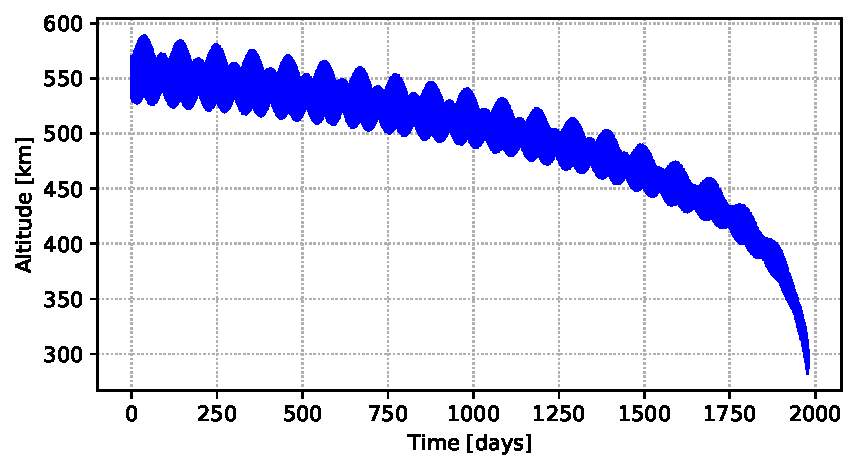
\includegraphics[width=0.8\columnwidth]{figures/lifetime}
        \end{center}
    \end{figure}

\end{frame}

\begin{frame}{Communication Study}

\end{frame}

\begin{frame}{Required Power Budget}

\end{frame}

\begin{frame}{Possible Solutions: Clock Reference}

    \begin{itemize}
        \item Quartz oscillator (XO)
        \item Temperature Compensated Crystal Oscillators (TCXO)
        \item Oven Controlled Crystall Oscillators (OCXO)
        \item Rubidium oscillators (RbXO)
        \item Cesium oscillators
        \item GPS disciplined oscillators (GPSDO)
    \end{itemize}

\end{frame}

\begin{frame}{Proposed Experiment}

    \begin{figure}[!ht]
        \begin{center}
            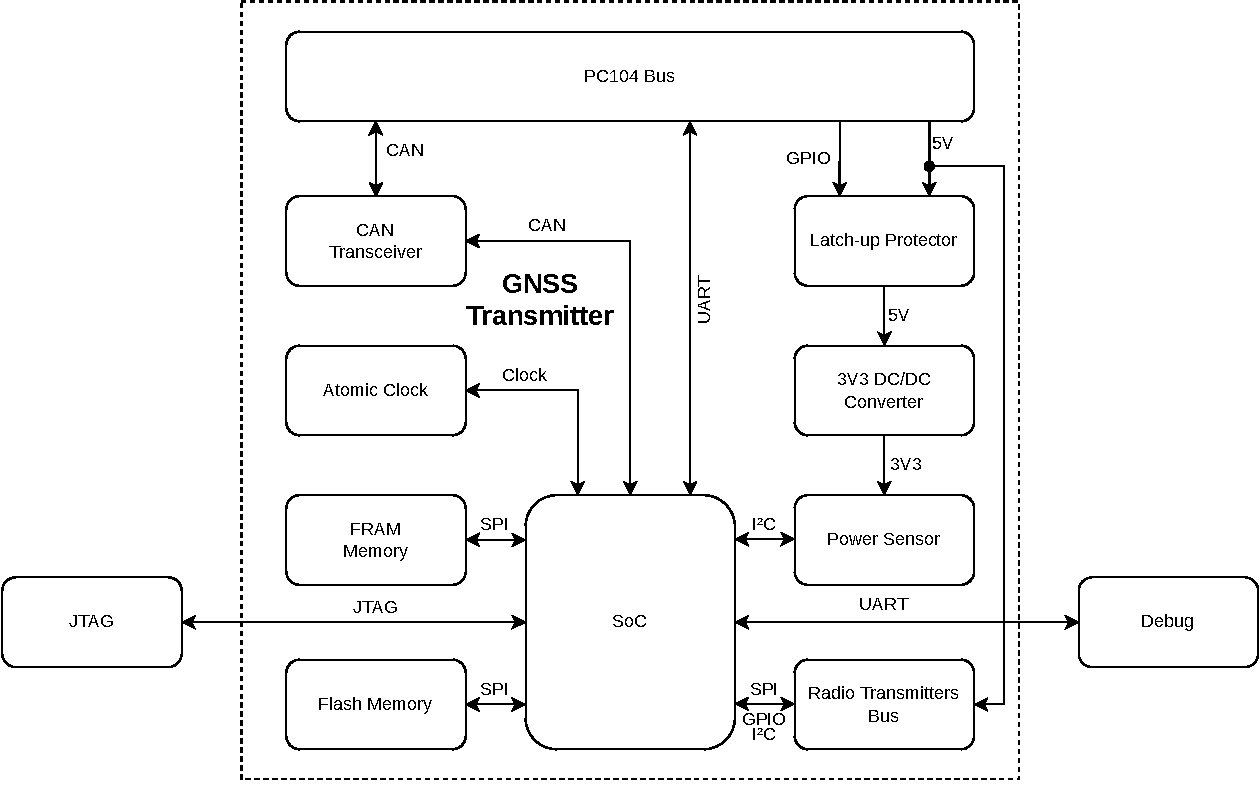
\includegraphics[scale=0.5]{figures/block-diagram}
        \end{center}
    \end{figure}

\end{frame}

\begin{frame}{Proposed Experiment}

    \begin{figure}[!ht]
        \begin{center}
            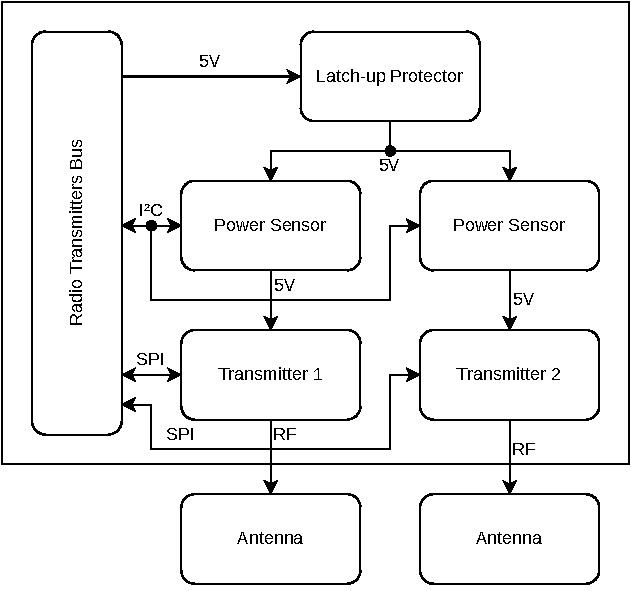
\includegraphics[scale=0.55]{figures/radios-block-diagram}
        \end{center}
    \end{figure}

\end{frame}
